\documentclass[12pt,a4paper]{article}
\usepackage[utf8]{inputenc}
\usepackage[T1]{fontenc}
\usepackage[french]{babel}
\usepackage{amsmath, amssymb}
\usepackage{graphicx}
\usepackage{geometry}
\geometry{margin=2cm}
\usepackage{enumitem}
\usepackage{float}
\usepackage{fancyhdr}
\usepackage{titlesec}
\usepackage{siunitx} % <-- AJOUTÉ : indispensable pour les commandes \SI
\pagestyle{fancy}


% Nettoyer les styles par défaut
\fancyhf{}

% En-têtes
\fancyhead[L]{Fiches d'exercices pour Maximilien (8)} % à gauche
\fancyhead[R]{Matteo Dubresson} % à droite

% Pieds de page
\fancyfoot[C]{\thepage} % numéro de page centré

%Titre et généralités
\title{Fiche d'exercices \\ pour Maximilien (8)}
\date{28/10/2026}
\author{}

%Espace entre les subsections
\titlespacing*{\subsection}{0pt}{5ex plus 0.5ex minus 0.2ex}{1.5ex plus 0.2ex}




\begin{document}

\maketitle


\subsection*{Exercice 1 : (Polynésie 2022)}


Dans les salles de spectacle, il existe des places appelées «~places aveugles~». Installé à ce type de place, un élève se rend compte que la qualité sonore du concert ne le satisfait pas.

L'objectif de cet exercice est d'étudier la diffraction des ondes lumineuses puis de montrer comment le phénomène de diffraction des ondes sonores permet de retrouver l'emplacement de l'élève dans la salle.

\bigskip
\textbf{Étude de la diffraction des ondes lumineuses}

En rentrant du concert, l'élève consulte une activité expérimentale sur la diffraction des ondes lumineuses dont voici un extrait : «~On dispose d'un laser de longueur d'onde inconnue $\lambda$ face à une fente de largeur $a$ réglable et d'un écran situé à une distance $D$ égale à \SI{2,00}{m} de la fente. On observe sur l'écran une figure de diffraction de tâche centrale de largeur $L$. Le schéma de la figure~1 modélise le montage réalisé.~»

% ---------- FIGURE 1 ----------
\begin{figure}[H]
  \centering
  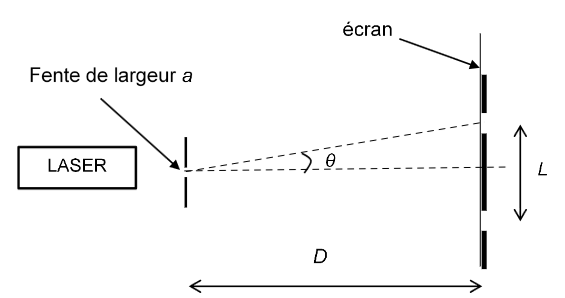
\includegraphics[width=0.6\textwidth]{image2.png} % <-- emplacement de la figure 1 (schéma du montage)
  \caption{Schéma du montage expérimental}
\end{figure}

L'angle caractéristique de diffraction $\theta$, en radian, a pour expression : $\theta = \dfrac{\lambda}{a}$. L'angle $\theta$ étant petit, on peut considérer que la valeur de la tangente de l'angle $\theta$ est égale à l'angle $\theta$ : $\tan\theta = \theta$.

\begin{enumerate}[label=\textbf{\arabic*.}, leftmargin=*, resume]
  \item Montrer que la largeur $L$ de la tâche centrale de diffraction a pour expression : $L = \dfrac{2\,\lambda\, D}{a}$.
\end{enumerate}

\bigskip
Lors de l'activité expérimentale, des mesures de la largeur $L$ de la tâche centrale de diffraction sur l'écran ont été effectuées en faisant varier la taille $a$ de la fente.
L'élève a ensuite obtenu le graphique de la figure~2.

% ---------- FIGURE 2 ----------
\begin{figure}[H]
  \centering
  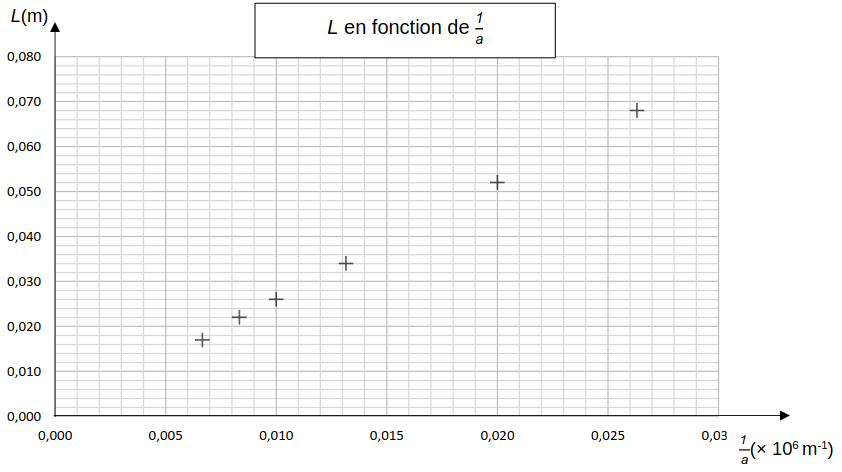
\includegraphics[width=0.9\textwidth]{image3.png}
  \caption{Graphique représentant la largeur de la tâche centrale $L$ en fonction de $\dfrac{1}{a}$}
\end{figure}

\begin{enumerate}[label=\textbf{\arabic*.}, leftmargin=*, start=2]
  \item À l'aide de la figure~2, montrer que la relation entre $L$ et $\dfrac{1}{a}$ est une équation linéaire de coefficient directeur $k$.
  \item Indiquer l'expression de $k$ en fonction de $\lambda$ et $D$.
  \item Montrer que la valeur de la longueur d'onde $\lambda$ est égale à \SI{6,5e-7}{m}.
\end{enumerate}

La valeur de l'angle $\theta_1$ correspondant à la fente de largeur $a_1 = \SI{38}{\micro m}$ est égale à \SI{1,7e-2}{rad}.

\begin{enumerate}[label=\textbf{\arabic*.}, leftmargin=*, start=5]
  \item Déterminer la valeur de l'angle $\theta_2$, en radian, correspondant à la fente de largeur $a_2$ égale à \SI{150}{\micro m}.
  \item En déduire que la diffraction est la plus marquée pour la fente de largeur $a_1$.
\end{enumerate}

\bigskip
\textbf{Étude de la diffraction des ondes sonores}

On rappelle que les caractéristiques de diffraction des ondes sont les mêmes pour les ondes lumineuses et les ondes sonores.

Lors du concert, l'élève constate qu'il perçoit mieux les sons graves de fréquence $f_1$ égale à \SI{200}{Hz} que les sons aigus de fréquence $f_2$ de valeur \SI{1,00}{kHz}.

\medskip
\textbf{Donnée :}
\begin{itemize}
  \item[$\blacktriangleright$] Vitesse du son dans l'air à la température de \SI{20}{\celsius} : $V_{son} = \SI{340}{m.s^{-1}}$
\end{itemize}

\begin{enumerate}[label=\textbf{\arabic*.}, leftmargin=*, start=7]
  \item Exprimer la longueur d'onde $\lambda$ d'une onde sonore en fonction de la vitesse du son $V_{son}$ et de sa fréquence $f$.
  \item Montrer que les longueurs d'onde $\lambda_1$ et $\lambda_2$ correspondant aux sons de fréquence $f_1$ et $f_2$ ont pour valeurs $\lambda_1 = \SI{1,70}{m}$ et $\lambda_2 = \SI{0,340}{m}$.
\end{enumerate}

% ---------- FIGURE 3 ----------
\begin{figure}[H]
  \centering% <-- emplacement de la figure 3 (scène, pilier, positions A, B, C)
  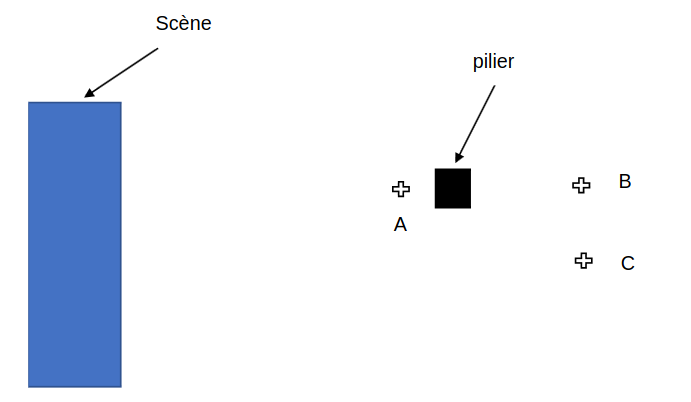
\includegraphics[width=0.6\textwidth]{image4.png}
  \caption{Schéma de la situation}
\end{figure}

La figure~3 ci-dessus représente la scène, un pilier de largeur voisine de \SI{70}{cm} et les positions possibles de l'élève lors du concert, repérées par les lettres A, B et C.
On admettra que la diffraction par le pilier est identique à celle créée par une fente de même largeur.

\begin{enumerate}[label=\textbf{\arabic*.}, leftmargin=*, start=9]
  \item En se référant à la figure~1 et à la réponse apportée à la question~8, choisir, en justifiant qualitativement, parmi les positions A, B ou C celle qui correspondrait le mieux à la situation décrite par l'élève lors du concert.
\end{enumerate}

\bigskip
\textbf{Étude de l'interférence des ondes sonores}

On suppose à présent une configuration ou le son sortirai à travers deux enceintes jusqu'à l'élève schématisé par le point M, coomme sur la figure si dessous, où on peut supposer que $a<<D$ : 

\begin{figure}[H]
  \centering% <-- emplacement de la figure 3 (scène, pilier, positions A, B, C)
  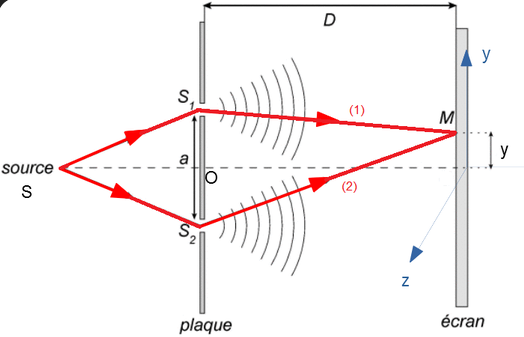
\includegraphics[width=0.6\textwidth]{image1.png}
  \caption{Schéma de la nouvelle situation}
\end{figure}

\begin{enumerate}[label=\textbf{\arabic*.}, leftmargin=*, start=10]
  \item En faisant l'hypothèse que les deux enceintes diffusent le son de manière cohérente, donner l'expression de la différence de marche $\delta$. 
  \item Pour un son de fréquence $f_1$ égale à \SI{1000}{Hz}, ou doit se placer l'élève par rapport à l'axe centralpour entendre un maximum de son ? Le minimum ? Justifier votre réponse.
\end{enumerate}

\newpage



\end{document}